\documentclass[10pt,twocolumn]{article}
\usepackage{fancyhdr, amsmath, amsthm, amssymb, hyperref, paracol, graphicx, setspace, lmodern}
\usepackage[margin=0.5in, top=0.8in,bottom=0.8in]{geometry}
\usepackage[version=3]{mhchem}
\newcommand{\scinot}[2]{#1\times 10^{#2}}
\newcommand{\bra}[1]{\left<#1\right|}
\newcommand{\ket}[1]{\left|#1\right>}
\newcommand{\dotp}[2]{\left<\left.#1\right|#2\right>}
\newcommand{\rd}[2]{\frac{d#1}{d#2}}
\newcommand{\pd}[2]{\frac{\partial #1}{\partial#2}}
\newcommand{\rtd}[2]{\frac{d^2#1}{d#2^2}}
\newcommand{\ptd}[2]{\frac{\partial^2 #1}{\partial#2^2}}
\newcommand{\norm}[1]{\left|\left|#1\right|\right|}
\newcommand{\abs}[1]{\left|#1\right|}
\newcommand{\Log}[0]{\mathrm{Log}}
\newcommand{\tensor}[1]{\overset{\leftrightarrow}{#1}}
\newcommand{\Arg}[0]{\mathrm{Arg}}
\newcommand{\Res}[0]{\mathrm{Res} }
\newcommand{\expvalue}[1]{\left<#1\right>}
\usepackage[labelfont=bf, font=scriptsize]{caption}
\everymath{\displaystyle}

\begin{document}

%\doublespace
\pagestyle{fancy}
\rhead{Yubo Su - Ma2a Final Revealed!}
%\setlength{\headheight}{15pt}

\begin{center}
    \textbf{All examples are harder than the actual problems on the final!}
\end{center}
\small

\section*{1)}

For the following system of differential equations
\begin{align*}
    \dot{x} &= -x + \frac{y}{2} + \cos^2 t\\
    \dot{y} &= -x - 2y + \sin t
\end{align*}
show that there exists a steady state and find it.

\section*{1s)}

Transform into a second-order equation as follows
\begin{align*}
    \ddot{y} &= -\dot{x} - 2\dot{y} + \cos t\\
    &= \underbrace{x + 2y - \sin t}_{-\dot{y}} + \sin t +\cos t - 2\dot{y} - \frac{5y}{2} - \cos^2 t \\
    &= -3\dot{y} - \frac{5y}{2} + \sin t +\cos t  - \frac{1+\cos 2t}{2}
\end{align*}

Now that it's linear in $y$, use undetermined coefficients! Ma2aNotes2 has this on page 10.

Note that we use undetermined coefficients for the three trig parts and that gives us the particular solutions. We then solve the inhomogenous case and add to it the three particular solutions that we find for each of the $g$. This is then the general solution for $L[y] = g = g_1 + g_2 + g_3$.

\section*{2)} 

Find the series solution to
$$x^2 y'' - x(1+x)y' + y = 0, x > 0$$
and identify it as an elementary function. Find the general solution.

\section*{2s)}

Refer to Frobenius Theory on LN3.24.2. First check that we satisfy orders of poles (divide through $x^2$), then find $\alpha = -1, \beta = 1$. We plug through indicial equation to find roots of $r^2 - 2r + 1 = 0, r_{1,2} = 1$. This means that we have a power series solution $y=x\sum_{n=0}^\infty a_nx^n$.

We now plug this back through the diffeq, computing $y' = \sum_{n=0}^\infty (n+1)a_n x^n$ and $y'' = \sum_{n=0}^\infty (n+1)na_nx^{n-1}$. Thus,
\begin{align*}
    \sum_{n=0}^\infty(n+1)na_nx^{n+1} - (1+x)\sum_{n=0}^\infty(n+1)a_nx^{n+1} + \sum_{n=0}^\infty a_nx^{n+1} &= 0\\
    \sum_{n=0}^\infty(n+1)na_nx^{n+1} - \sum_{n=0}^\infty(xn + x + n)a_nx^{n+1}&= 0\\
    \sum_{n=0}^\infty(n)na_nx^{n+1} - \sum_{n=0}^\infty(n + 1)a_nx^{n+2}&= 0\\
    \sum_{n=0}^\infty(n)na_nx^{n+1} - \sum_{n=1}^\infty na_{n-1}x^{n+1}&= 0
\end{align*}
which then gives $na_n = a_{n-1}$ and solution $xe^x$. We can then reduction of order to find the general solution.

\section*{3)}

Find all solutions to
$$\ptd{u}{t} + \pd{u}{t} + u = \ptd{u}{x}$$
with $u(x,t) = X(x) T(t)$ subject to $X(0) = 0, X(\pi) = 0$.

\section*{3s)}

Plug and chug the separation of variables to obtain $\ddot{T}X + \dot{T}X + TX = TX''$. This then gives that
$$\frac{\ddot{T} + \dot{T} + T}{T} = \frac{X''}{X} = -\lambda$$
where $-\lambda$ is some constant (sign chosen with foresight), because in order for the two to be identically equal even though separated variables it's clear they must both be constant. 

We then solve the BVP $X'' = -\lambda X, X(0) = X(\pi) = 0$ and have $X_n = \sin nx$ eigenvectors. Plugging this through with $\lambda = n^2$ eigenvalues we then solve
$$\ddot{T}_n + \dot{T}_n + T_n = -n^2T_n$$
which yields solutions $T_n(t) = A_ne^{-t/2}\cos \left( t\sqrt{n^2+\frac{3}{4}} \right) + B_ne^{-t/2}\sin\left( t\sqrt{n^2 + \frac{3}{4}} \right)$. The total solutions are then $X_n(x) T_n(t)$.

\section*{4)}

Given system
\begin{align*}
    \dot{x} &= x(1-x-2y)\\
    \dot{y} &= y(1-y-2x)
\end{align*}

\begin{itemize}
    \item Find all singular points in $\left\{ x \geq 0, y \geq 0 \right\}$ and identify the type of point and stability through linearization.
    \item Find the eigenvectors for singular points.
    \item Draw phase portrait.
    \item $x(0) = 1, y(0) = 2$ - determine limiting behavior $t \to \infty$.
\end{itemize}

\section*{4s)}

Upon careful inspection we find singular points $(0,0), (1,0), (0,1), \left( \frac{1}{3}, \frac{1}{3} \right)$. We can then compute the Jacobian matrix
$$\begin{pmatrix} \pd{\dot{x}}{x} & \pd{\dot{x}}{y}\\ \pd{\dot{y}}{x} & \pd{\dot{y}}{y} \end{pmatrix}  = \begin{pmatrix} 1-2x & -2x \\ -2y & 1-2y \end{pmatrix}$$

At each of the four singular points, these are then
\begin{align*}
    (0,0) &= \begin{pmatrix} 1&0\\0&1 \end{pmatrix}\\
    (1,0) &= \begin{pmatrix} -1&0\\-2&-1 \end{pmatrix} \\
    (0,1) &= \begin{pmatrix} -1&-2\\0&-1 \end{pmatrix} \\
    \left( \frac{1}{3}, \frac{1}{3} \right) &= \begin{pmatrix} -\frac{1}{3} & -\frac{2}{3}\\-\frac{2}{3}&-\frac{1}{3} \end{pmatrix}
\end{align*}

Solving our eigenvalues we find that $(0,0)$ has two positive eigenvalues and so is an unstable star. We find that $(1,0),(0,1)$ have repeated negative real eigenvalues that are non multiples of the identity so we have a stable irregular node. The last point has eigenvalues of opposite sign and so is a saddle point. If we also consider our eigenvectors, we'll have a plot that looks roughly like the below
\begin{figure}[!h]
    \centering
    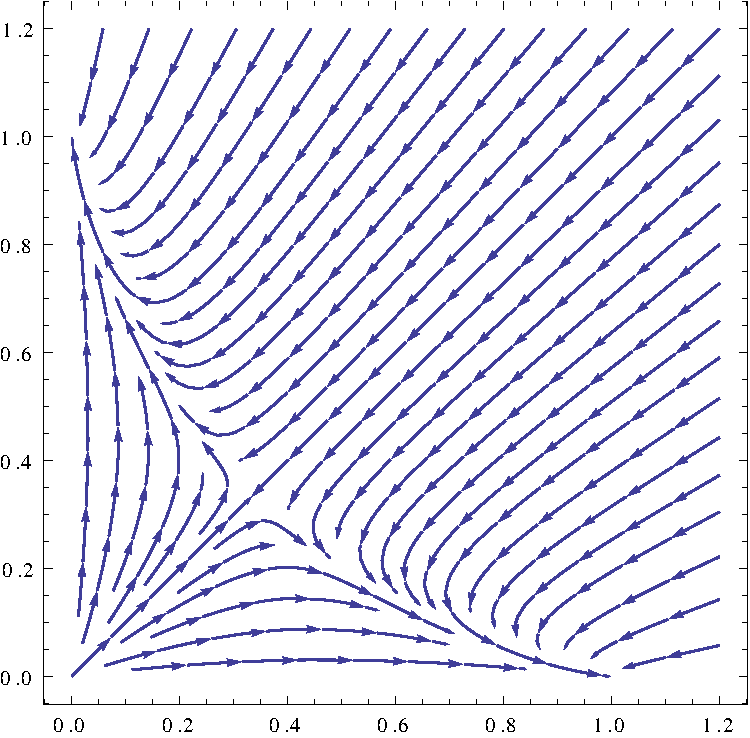
\includegraphics[scale=0.3]{Ma2aFinal4Phase.pdf}
    \caption{Non-linearized, generated by Mathematica. Note critical point behavior.}
\end{figure}

We then want the limiting behavior as $t \to \infty$ when $x(0) = 1, y(0) = 2$. Makarov doesn't cover this in class, but the limiting behavior is obviously to $(0,1)$ either by inspection of phase portrait or by copious argumentation.

\section*{5)}

Consider a particle of unit mass moving in potential $U(x) = x-x^3$ so that $\ddot{x} = -U'(x) = 3x^2 - 1$.
\begin{enumerate}
    \item Draw phase portrait.
    \item Find periods of small oscillations.
    \item Write down the equation of motion in the presence of a damping coefficient $-\dot{x}$ and draw the phase portrait.
\end{enumerate}

\section*{5s)}

Let $y = \dot{x}$, so our system becomes
\begin{align*}
    \dot{x} &= y\\
    \dot{y} &= 3x^2 - 1
\end{align*}

We note critical points at $y=0, x = \pm \sqrt{\frac{1}{3}}$. We write our Jacobian matrix
$$\begin{pmatrix} 0&1\\6x & 0 \end{pmatrix} $$

We then note that about $x = \sqrt{\frac{1}{3}}$ we have opposite sign real eigenvalues which gives a saddle point. About the other point we have complex eigenvalues $\pm i \sqrt{2}$ which suggests oscillations. Then writing the eigenvalues of the Jacobian as $\pm i\omega$ at both critical points we know that the period of small oscillations about these critical points is given $T = \frac{2\pi}{\omega}$ (by LN4 34.3). 

We draw phase portrait by simply drawing the saddle point and then giving the centre the correct rotation direction. The Mathematica version is 
\begin{figure}[!h]
    \centering
    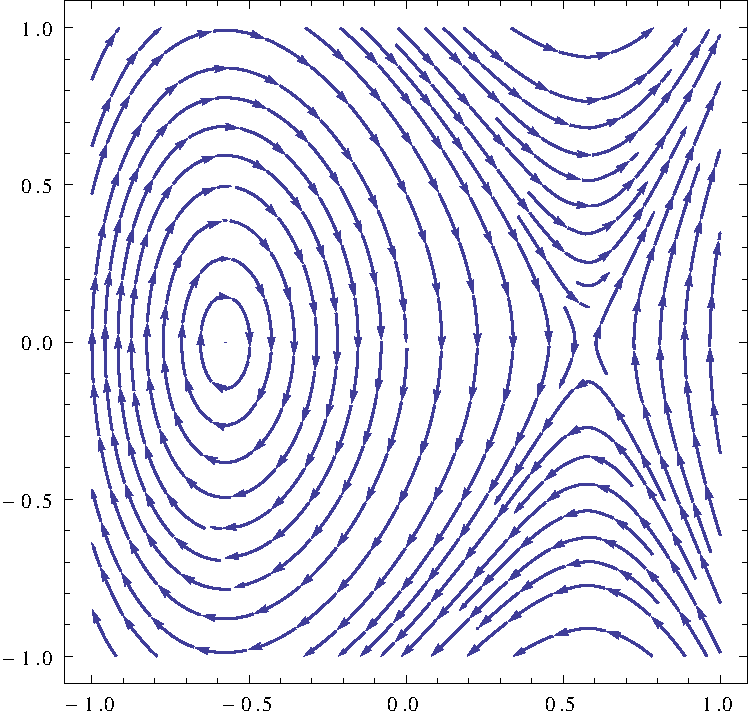
\includegraphics[scale=0.3]{Ma2aFinal5Phase.pdf}
    \caption{Non-linearized, generated by Mathematica. Note oscillatory behavior.}
\end{figure}

We then add in dissipation (via a $-y$ term in the $\dot{y}$ equation) and note that it has the same stationary points, as we expect. The equations then become
\begin{align*}
    \dot{x} &= y\\
    \dot{y} &= 3x^2 -y - 1
\end{align*}

The phase portrait is then
\begin{figure}[!h]
    \centering
    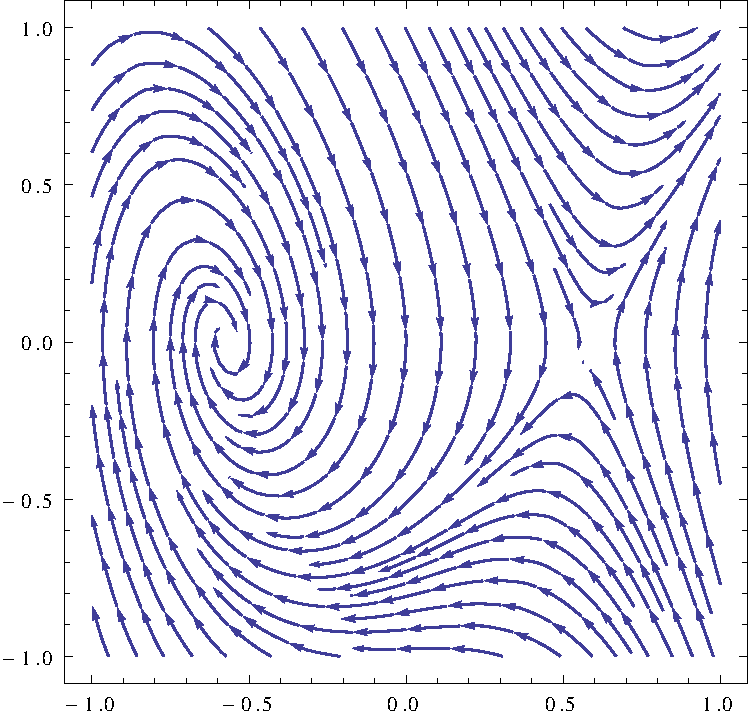
\includegraphics[scale=0.3]{Ma2aFinal5bPhase.pdf}
    \caption{Non-linearized, generated by Mathematica. Note damping.}
\end{figure}

\section*{6)}

Determine whether the critical point of the system
\begin{align*}
    \dot{x} &= 2y - x - y^3 + y^4\\
    \dot{y} &= x - 2y
\end{align*}
is stable or unstable (Hint: use Lyapunov equations).

\section*{6s)}

We note that $x = y = 0$ is a critical point of the system. We note also that $y=1, x=2$ is the only other critical point; setting $\dot{y} = \dot{x} = 0$ produces $y^4 - y^3 = 0$ and the only solutions are $y=0, y=1$.

We then seek the Lyapunov equation about $x=y=0$. We take general form $\Phi(x,y) = x^m + y^n$ which yields directional derivative
$$mx^{m-1}\left( 2y - x - y^3 + y^4 \right) + ny^{n-1}\left( x-2y \right)$$

We require $(0,0)$ to be at least strictly nonpositive. 

\end{document}
